\documentclass[12pt]{article}
\usepackage[margin=1in]{geometry}
\usepackage{textcomp}
\usepackage{multirow}
\usepackage{graphicx}
\pagestyle{empty}

\setlength{\parskip}{\baselineskip}
\setlength{\parindent}{0pt}

\begin{document}
\begin{center}
\large Control Rod Worth Calibration \\
\normalsize Generated \today
\end{center}

\emph{Control rod worths}

\begin{tabular}{r c}
	Safe Rod & \textbf{\$2.41} \\
	Shim Rod & \textbf{\$3.61} \\
	Reg Rod & \textbf{\$1.30} \\ \hline
	Total & \textbf{\$7.33}
\end{tabular}

\emph{Peak reactivity addition rates for each control rod}

\begin{tabular}{r c c c c}
	& Max.\ Add.\ Rate & Max.\ Add.\ Rate & Spec & OK? \\
	Safe & \textbf{3.35 \textcentoldstyle/\%} & \textbf{6.82 \textcentoldstyle/sec} & $< 12$ \textcentoldstyle/sec & \textbf{OK} \\
	Shim & \textbf{4.10 \textcentoldstyle/\%} & \textbf{5.27 \textcentoldstyle/sec} & $< 12$ \textcentoldstyle/sec & \textbf{OK} \\
	Reg & \textbf{1.94 \textcentoldstyle/\%} & \textbf{5.33 \textcentoldstyle/sec} & $< 12$ \textcentoldstyle/sec & \textbf{OK}
\end{tabular}

Plots of the original data, and polynomials of best fit, are on the next page.

\emph{Core excess and shutdown margin}

The core excess is calculated twice: once using the Safe Rod at its lowest critical point with the other two rods removed, and once using the Shim Rod in the same configuration. Both values of the CXS are given here; they should be nearly equal.

The shutdown margin and one-stuck-rod SDM are also calculated using each value of the CXS. For the ``one stuck rod'' rule, we assume that the most reactive control rod, in this case the \textbf{Shim Rod}, is completely withdrawn.

\begin{tabular}{r c c c c}
	& Safe & Shim & Spec & OK? \\
	CXS height & \textbf{47.3\%} & \textbf{51.4\%} & --- & --- \\
	Core excess & \textbf{\$1.35} & \textbf{\$1.35} & $< \$3.00$ & \textbf{OK} \\
	Shutdown margin & \textbf{\$5.97} & \textbf{\$5.97} & $> \$1.00$ & \textbf{OK} \\
	One-stuck-rod SDM & \textbf{\$2.36} & \textbf{\$2.36} & $> \$0.50$ & \textbf{OK}
\end{tabular}

\begin{tabular}{c c c}
	\underline{\hspace{3in}} & {\Large /} & \underline{\hspace{1in}} \\
	Operator Signature & & Date
\end{tabular}

\newpage
\newgeometry{margin=0.5in}
\begin{center}
    \begin{tabular}{c c}
    \multicolumn{2}{c}{\textbf{Safe Rod}} \\
    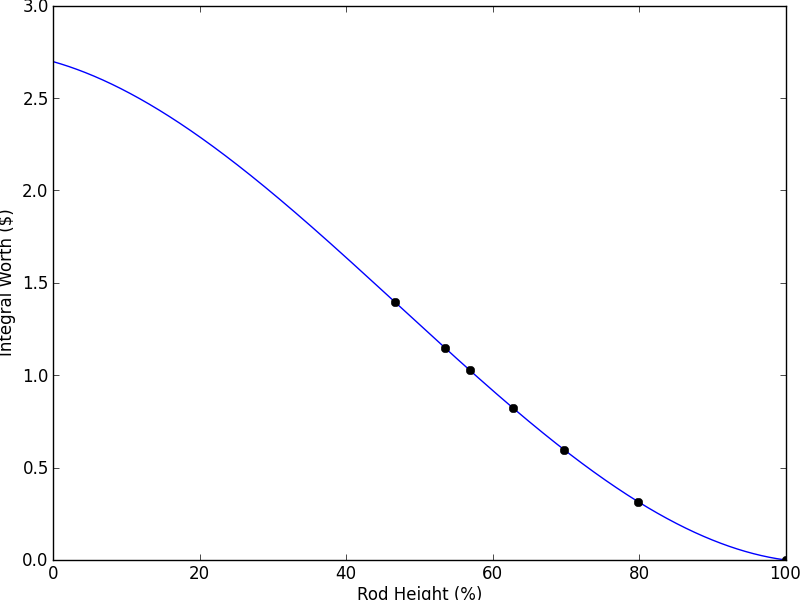
\includegraphics[width=3.2in]{safe-integral} & 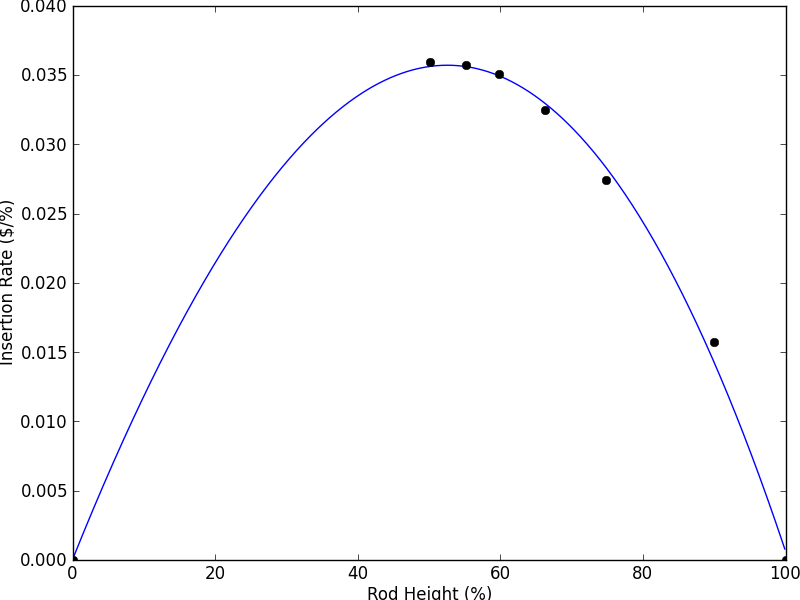
\includegraphics[width=3.2in]{safe-rate} \\
    \multicolumn{2}{c}{\textbf{Shim Rod}} \\
    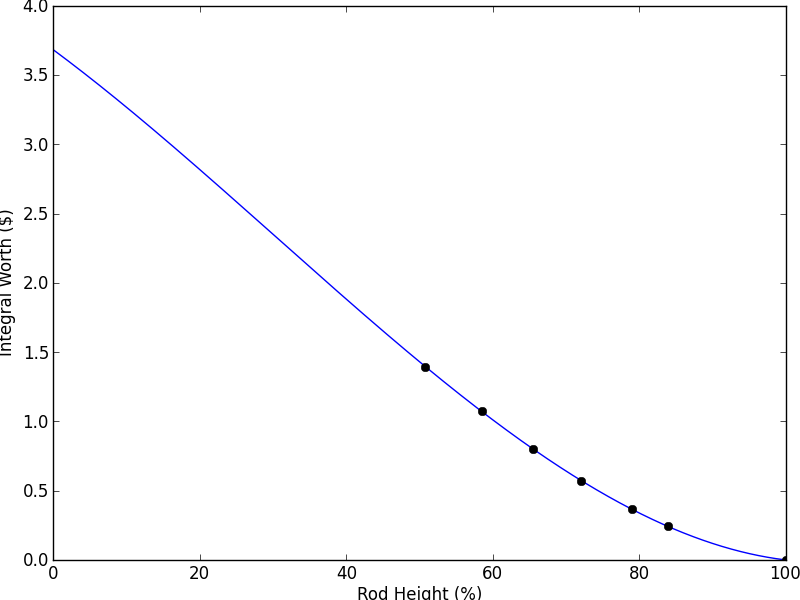
\includegraphics[width=3.2in]{shim-integral} & 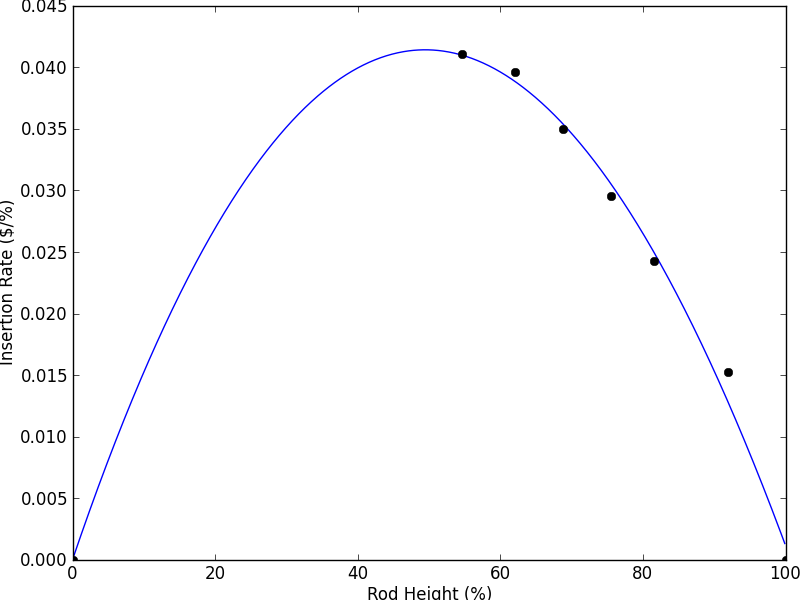
\includegraphics[width=3.2in]{shim-rate} \\
    \multicolumn{2}{c}{\textbf{Reg Rod}} \\
    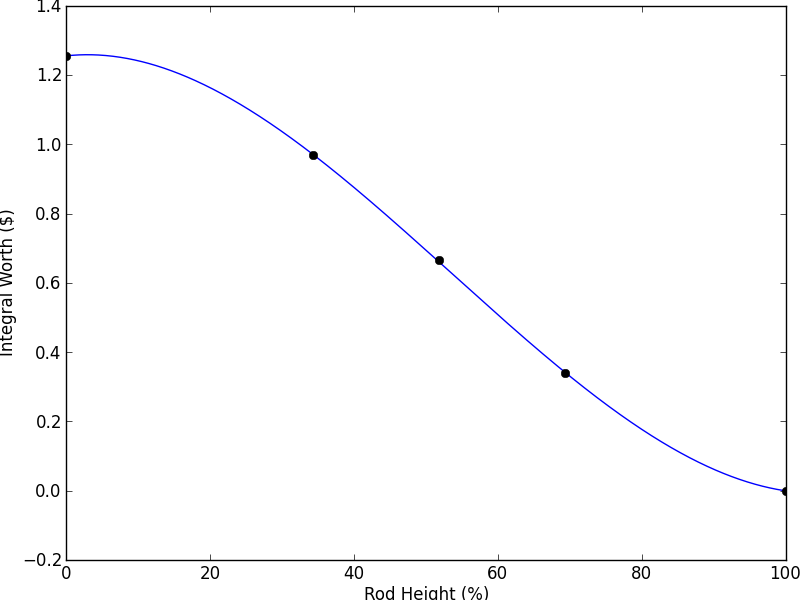
\includegraphics[width=3.2in]{reg-integral} & 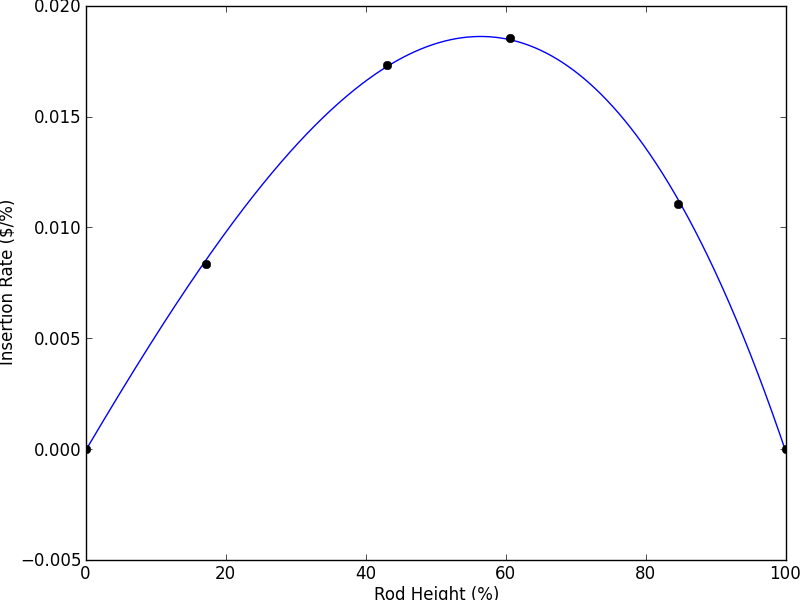
\includegraphics[width=3.2in]{reg-rate} \\
    \end{tabular}
\end{center}

\begin{tabular}{r l}
Safe Int. Worth: & $(3.98273 \times 10^{-6})\, x^3 + -0.000619558 \, x^2 + -0.00198042 \, x + 2.41087 $ \\
Safe Add. Rate:  & $(-6.41211 \times 10^{-8})\, x^3 + (-3.38634 \times 10^{-6})\, x^2 + 0.000987919 \, x + (4.67726 \times 10^{-5})$ \\
Shim Int. Worth: & $(2.8531 \times 10^{-6})\, x^3 + -0.000271281 \, x^2 + -0.0375282 \, x + 3.61306 $ \\
Shim Add. Rate:  & $(8.51371 \times 10^{-9})\, x^3 + (-1.74377 \times 10^{-5})\, x^2 + 0.00166952 \, x + (1.77775 \times 10^{-5})$ \\
Reg Int. Worth:  & $(2.43602 \times 10^{-6})\, x^3 + -0.000400405 \, x^2 + 0.00266296 \, x + 1.30132 $ \\
Reg Add. Rate:   & $(-5.11924 \times 10^{-8})\, x^3 + (1.28723 \times 10^{-7})\, x^2 + 0.000499231 \, x + (-1.64335 \times 10^{-5})$ \\
\end{tabular}
\end{document}
